\subsection{$\Sigma$-encoding for Conformance Checking}
\label{sec:dadtap}
As per the previous considerations, we want to show that, to solve the trace alignment problem for data-aware declarative conformance checking, it is sufficient to provide a specific characterization of $\Sigma$. $\Sigma$ will be used to generate an automaton accepting symbols in $\Sigma$ and the automaton will be used to test log traces represented as finite sequences in $\Sigma^*$. The proposed approach for obtaining $\Sigma$ from a (data-aware) Declare model $\mathcal{M}$ is sketched in Figure~\ref{fig:twoexamples}, and described in detail in the following.

\begin{table*}[!t]
	\centering
	\captionsetup[subtable]{position = below}
	\captionsetup[table]{position=top}
	\caption{Intermediate steps for generating distinct atoms for \texttt{B} labeled events by partitioning the data space via intervals in Declare clauses.}
	\begin{subtable}{0.45\linewidth}
		\centering
		\resizebox{\textwidth}{!}{%
						\begin{tabular}{c|c||c|c|}
				\toprule
				\multicolumn{2}{c||}{$\mu(\texttt{B},x)$} & \multicolumn{2}{c}{$\mu(\texttt{B},y)$}\\
				\midrule
				$\texttt{B}.x>3$      & $\texttt{B}.x>3$ & $\texttt{B}.y=0$ & $0\leq \texttt{B}.y\leq 0$\\
				$\texttt{B}.x> 0$ & $0<\texttt{B}.x\leq 3$, $ \texttt{B}.x>3$ & $\texttt{B}.y\neq 0$ & $\texttt{B}.y<0\vee \texttt{B}.y>0$\\
				$\texttt{B}.x\leq 0$ & $ \texttt{B}.x\leq 0$ & & \\
				\bottomrule
			\end{tabular}%
		}
		\caption{Interval decomposition in $\mu(\cdot, \cdot)$}
		\label{tab:dimFFT}
	\end{subtable}\quad
	\begin{subtable}{0.6\linewidth}
		\centering
		\resizebox{.5\textwidth}{!}{%
			\begin{tabular}{c|ccc}
	\toprule
	\texttt{B} & $\texttt{B}.y< 0$ & $\texttt{B}.y=0$ & $\texttt{B}.y>0$ \\
	\midrule
	$\texttt{B}.x\leq 0$ & $p_1$ & $p_2$ & $p_3$   \\
	$0<\texttt{B}.x\leq 3$ & $p_4$ & $p_5$ & $p_6$\\
	$\texttt{B}.x>3$ & $p_7$ & $p_8$& $p_9$ \\
	\bottomrule
\end{tabular}%
		}
		\caption{Atom generation for \texttt{B} by data space partitioning via $\times_{k\in K}\mu(\texttt{B},k)$}
		\label{tab:dimGMM}
	\end{subtable}
\vspace{-1cm}
\end{table*}

\begin{figure}[!t]
	\centering
	%{\hspace{-1.3cm}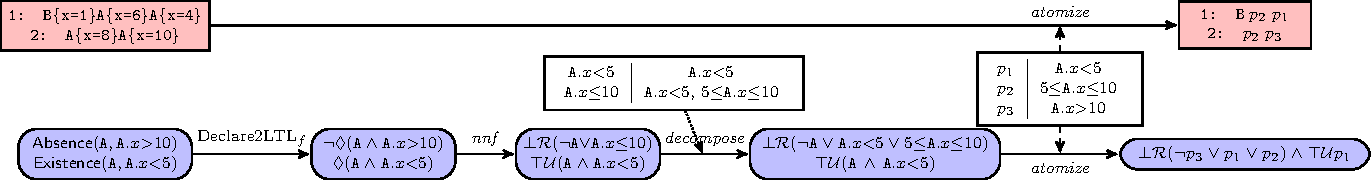
\includegraphics[width=1.3\textwidth]{images/example_1}}
	{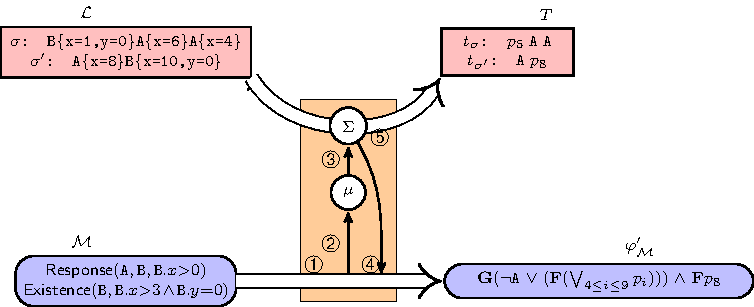
\includegraphics[width=.6\textwidth]{images/example_3}}
	\caption{Intermediate steps required for obtaining $\Sigma=\Set{p_i|1\leq i\leq 9}\cup\{\texttt{C}\}$ from $\mathcal{M}$ and transforming $\mathcal{L}=\Set{\sigma,\sigma'}$ into a set of finite sequences $T=\Set{t_\sigma,t_{\sigma'}}$, as well as replacing atoms in $\varphi_{\mathcal{M}}$ with equivalent atoms in $\Sigma$ ($\varphi_{\mathcal{M}}'$).}\label{fig:twoexamples}
\vspace{-.5cm}
\end{figure}

In the first \emph{Declare2LTL}$_f$ step, we exploit the usual conversion of each single Declare clause into an LTL$_f$ formula (see Table 1) in the \textit{negated normal form} \cite{LiPZVR20}, where negations are possibly pushed inside atoms ``$\texttt{A}.k\;\Re\; c$'' by replacing $\Re$ with its negation.
\begin{ex} \label{ex:first}
The Declare model $\mathcal{M}$ containing clauses $\mathsf{Response}(\texttt{C},\texttt{B},\;\texttt{B}.x>0)$ and
$\mathsf{Existence}(\texttt{B},\; \texttt{B}.x>3\wedge \texttt{B}.y=0)$ is represented as the intermediate LTL$_f$ formula $\varphi_{\mathcal{M}}=\lglobally(\neg\texttt{C}\vee \lfuture(\texttt{B}\wedge \texttt{B}.x>0))\wedge \lfuture(\texttt{B}\wedge \texttt{B}.x>3\wedge \texttt{B}.y=0)$.
\end{ex}

In the second \textit{decomposition} step, for each compound condition $\psi=\texttt{A}\wedge \phi^d$ over labels $\texttt{A}\in\textsf{Act}$, we collect all the atoms in $\phi_d$ in the form ``$\texttt{A}.k\;\Re\; c$'' for each $k\in K$ in a map $\mu(\texttt{A},k)$. Contextually, we represent atoms as intervals, and we \textit{decompose} them
%
%%We now describe the main contribution of the paper, namely a technique for computing log trace alignments over Declare data-aware models. Our approach takes as input \begin{enumerate*}[label=\emph{\alph*})]
%	\item a Declare data-aware model $\mathcal{M}$ expressed as a set of instantiated templates,
%	\item a log trace $\sigma$,
%\end{enumerate*} and ranks the outcome of a LTL$_f$ conformance checking $\sigma\tilde{\vDash}\varphi$ accordingly to a data distance function $\mathcal{D}$.
%
%%The input transformation for reducing the data-aware alignment problem to the data-agnostic one is presented in Figure~\ref{fig:twoexamples} for two alignment examples. In particular, we first transform the data-aware Declare model, for then collecting the required information for providing the trace transformation.
%
%%\textbf{data-aware Declare Model Processing.}
%
%
%
%
%%In step 3, we collect the data-aware predicates ``$\texttt{A}.\textit{var}\;\Re\;c$'' from all the model's clauses and group them by $\texttt{A}.\textit{var}$; each of these predicates is \textit{decomposed}
into a disjunction of maximal non-overlapping data-aware predicates. This task can be efficiently computed via interval trees \cite{inttree}. Last, we replace the atoms in each LTL$_f$ formula by its decomposed representation.%, if any.
\begin{continueexample}{ex:first}\label{ex:second}
Table~\ref{tab:dimFFT} shows the interval decomposition results for the $\psi$ extracted from $\mathcal{M}$. E.g., predicates $\texttt{B}.x>3$ and $\texttt{B}.x>0$ are first represented as intervals $\interval({3,+\infty})$ and $\interval({0,+\infty})$, and then decomposed into disjoint sub-intervals $\interval({-\infty,0}]$, $\interval({0,3}]$, and $\interval({3,+\infty})$. As a result, $\varphi_{\mathcal{M}}$ is decomposed into $\varphi_{\mathcal{M}}^d=\lglobally(\neg\texttt{C}\vee \lfuture(\texttt{B}\wedge \texttt{B}.x>0))\wedge \lfuture(\texttt{B}\wedge (0<\texttt{B}.x\leq 3\vee \texttt{B}.x> 3) \wedge \texttt{B}.y=0)$.
\end{continueexample}

In the third \textit{atomization} step, we put an atom $\texttt{A}\in\textsf{Act}$ in $\Sigma$ if the map $\mu(\texttt{A},k)$ is empty for each key $k\in K$; otherwise, given all the keys $k_{\texttt{A}_1},\dots,k_{\texttt{A}_h}\in K$ for which the map $\mu(\texttt{A},k_{\texttt{A}_i})$ is not empty, we partition the data space by combining the non-overlapping intervals obtained from the previous step as $\mu(\texttt{A},k_{\texttt{A}_1})\times\cdots\times\mu(\texttt{A},k_{\texttt{A}_h})$. For each of these interval combinations, we generate a fresh atom and put it in $\Sigma$.
\begin{continueexample}{ex:first}
Label \texttt{C} is never associated to a data condition, and therefore it will be associated to one single atom \texttt{C}. On the other hand, label \texttt{B} is associated to several atoms obtained by partitioning the data space via the intervals in Table~\ref{tab:dimFFT}. Table~\ref{tab:dimGMM} shows the atom decomposition of \texttt{B} via data intervals over keys $x$ and $y$, which induce a space partitioning of 9 intervals, for which we generate nine distinct atoms $p_1\dots p_9$. As a result, we obtain $\Sigma=\Set{p_i|1\leq i\leq 9}\cup\Set{\texttt{C}}$ in Figure~\ref{fig:twoexamples}.
\end{continueexample}


%In step 4, for each event label \texttt{C}, we partition the data space \textit{var}$_1\times\dots\times$\textit{var}$_h$ associated to \texttt{C} by exploiting the disjoint intervals mined in the previous step. Each of such combination will be syntactically represented as a fresh \textit{atom}  proposition $p_i$: this implies that the label \texttt{C} is represented by the disjunction $\bigvee_ip_i$. When the data space associated to the predicates mined for \texttt{C} has only one property,  the atoms corresponds to the ones mined in the previous step. E.g., \texttt{C} in the first example from \ref{fig:twoexamples} is equivalent to $p_1\vee p_2\vee p_3$, and $\texttt{C}.\textit{x}<5$ is rewritten as $p_1$; given that such atoms represent disjoint intervals, then $\texttt{C}\wedge p_1\equiv p_1$. Similarly, $\neg \texttt{C}\vee \texttt{C}.\textit{x}<5\vee 5\leq\texttt{C}.\textit{x}\leq 10$ can be immediately rewritten as $\neg(p_1\vee p_2\vee p_3)\vee p_1\vee p_2$, which is equivalent to $\neg p_3\vee p_1\vee p_2$. Last, each LTL$_f$ representation of a data-aware Declare clause is represented into one si\ding{193}ngle LTL$_f$ formula by conjunction and simplification.


Starting from these atoms, we firstly replace the compound conditions in the LTL$_f$ interpretation $\varphi_{\mathcal{M}}$ of $\mathcal{M}$ with a disjunction of atoms from $\Sigma$ as described in Table~\ref{tab:dimGMM}, thus obtaining an equivalent LTL$_f$ formula $\varphi_{\mathcal{M}}'$. Secondly, we generate a finite sequence $t_\sigma\in T$ for each log trace $\sigma\in\mathcal{L}$ by replacing each event $\sigma_i$ in $\sigma$ with the only atom $t_i\in \Sigma$ such that $\sigma_i\vDash t_i$.
%
%\textbf{data-aware Log Trace Processing.} Given the atomization in Step 4, we process each data-enriched event within the trace as follows: if the event label is never associated with a data predicate, then we just discard the data information; otherwise, we replace each event with the single corresponding atom satisfying the associated semantics. Please observe that, by previous construction, each event can be represented by just one possible propositional atom, as the previous construction guarantees a partitioning (thus non-overlapping) representation of the data space.

\begin{continueexample}{ex:first}
With reference to our running example, we replace the compound conditions in $\varphi_{\mathcal{M}}^d$ with the previously generated atoms; the compound condition $\texttt{B}\wedge \texttt{B}.x>0$ is replaced by all the possible configurations of $y$ and data intervals $0<\texttt{B}.x\leq 3$ and $\texttt{B}.x>3$, which are identified by the disjunction $p_4\vee p_5\vee p_6\vee p_7\vee p_8\vee p_9$. On the other hand, $\texttt{B}\wedge\texttt{B}.x>3\wedge \texttt{B}.y=0$ can be directly replaced by atom $p_8$: this results into an equivalent formula $\varphi_{\mathcal{M}}'=\lglobally(\neg\texttt{C}\vee(\lfuture(p_4\vee p_5\vee p_6\vee p_7\vee p_8\vee p_9)))\wedge \lfuture p_8$.
Given a log $\mathcal{L}=\{\texttt{B\{x=1,y=0\}C\{x=6\}C\{x=4\}},
\texttt{ C\{x=8\}B\{x=10,y=0\}}\}$,
all the events labeled as \texttt{C} are replaced with atom \texttt{C}, as there are no (data) conditions related to \texttt{C} in $\mathcal{M}$ that we can exploit to partition the data space. On the other hand, each event labeled as \texttt{B} is replaced by an equivalent atom in $\Sigma$: event \texttt{B\{x=1,y=0\}} is uniquely represented by $p_5$, while event \texttt{B\{x=10,y=0\}} is uniquely represented by $p_8$. %Similar considerations can be drawed for the $\psi$ compound atoms in $\varphi_{\mathcal{M}}$ where compound conditions are replaced into an equivalent disjunction of atoms in $\Sigma$:
This transformation results into a set of string sequences $T=\{{ p_5\;\texttt{C\;C}}, \texttt{C}\;p_8\}$.
\end{continueexample}


After generating $\varphi_{\mathcal{M}}'$, we can exploit existing approaches \cite{Westergaard11} to generate a DFA that only accepts sequences satisfying $\varphi_{\mathcal{M}}'$. With reference to the previous example, the first trace is not conformant to $\mathcal{M}$, since the first sequence is not accepted by the associated automaton. Similarly, the second trace is conformant to $\mathcal{M}$, since the second sequence is accepted by the associated DFA. In the forthcoming subsection, we will discuss how to generate repaired sequences that are accepted by the reference model.

\subsection{Automaton Manipulation for Trace Alignment}\label{ssec:amfta}
Consider a sequence $t_\sigma=t_1\cdots t_n$ generated from a trace $\sigma$, and the constraint automaton $\mathcal{A}_{\varphi_{\mathcal{M}}}$ generated from the Declare model $\mathcal{M}$. If the trace is deviant with respect to the model, we are interested in generating a repair sequence $\varrho=\varrho_1\cdots \varrho_m$ from $t_\sigma$ describing the operations to perform over $\sigma$ to make it conformant to $\mathcal{M}$.

To realize this transformation, we consider two types of atomic violations, which can be caused by wrong (\textit{deletion}) or missing (\textit{insertion}) atoms in $\Sigma$. Differently from the non-data aware case \cite{XuLZ17a}, we also need to model \textit{replacement} operations, defined as a data update within one single trace event: these operations can be mimicked by a delete operation followed by an insertion, as they substitute an event within a trace with the same event where a data value has been updated. The above operations\added{, that will be later on encoded as PDDL actions,} can be defined as follows:
\begin{itemize}
	%\item synchronization $[\sigma_k\leftrightarrow \phi]$ aborts if $\sigma_k\neq\phi$, for  $1\leq k\leq |\sigma|$
	\item \textit{deletion}/\texttt{del} $[\#\sigma_k\leftarrow \phi]::= \sigma_1\cdots\sigma_{k-1}\sigma_{k+1}\cdots \sigma_n$,\,\,\, for $n=|\sigma|$, $1\leq k\leq n$, and $\phi=\sigma_k$
	\item \textit{insertion}/\texttt{ins} $[@\sigma_k\leftarrow \phi]::= \sigma_1\cdots\sigma_{k-1}\phi\sigma_{k}\cdots \sigma_n$,\,\,\,\,\,\,\,\,\,\,\,\, for $n=|\sigma|$ and $1\leq k\leq n$
	\item \textit{replacement}/\texttt{repl} $[\sigma_k[\phi\mapsto\phi']]::=\sigma_1\cdots \sigma_{k-1}\phi'\sigma_{k+1}\cdots\sigma_n$ for $n=|\sigma|$, $1\leq k\leq n$, and $\phi=\sigma_k$
\end{itemize}
\added{Similarly to customary cost-based trace aligners,} each of these operations has an associated cost, either quantifying the severity of the found violation or determining which operations shall be preferred. E.g., by assigning a higher cost to insertions and deletions and a lower one to replacements, we will favor replacements when possible. The \textit{alignment cost} is defined as the number of deletions multiplied by their cost, plus the number of insertions multiplied by their cost, plus the number of replacements multiplied by their cost.

We can now define the conformance checking problem as follows:
\begin{definition}[Log/Declare Conformance Checking]
Given a trace $\sigma$ and a Declare model $\mathcal{M}$, checking the conformance of $\sigma$ against $\mathcal{M}$ is the task of verifying if $\sigma$ conforms to $\mathcal{M}$, or $\sigma$ is deviant and \added{there} exists a repair sequence $\varrho$ making $\sigma$ non-deviant for $\mathcal{M}$ and guaranteeing a minimal transformation cost.
\end{definition}

%\texttt{\color{red}[TODO]} we consider insertions and deletions as possible repairs, while substitutions can be modeled by deletions followed by insertions. Synchronizations are \texttt{noops} requiring that a trace $\sigma$ at step $k$ contains a predicate $\phi$.
%%
%Therefore, any repair  of a trace $\sigma$ can be expressed in terms of a sequence of operations $\texttt{op}_1\cdots \texttt{op}_m$ which, when executed in appearance order, generate a novel trace $\tilde{\sigma}$ from $\sigma$.  \texttt{\color{red}[TODO]}
%%
%
%Last, the amount of repairs can be numerically quantified using a cost function $\mathcal{C}$ returning zero for any synchronization and $1$ otherwise; therefore $cost(\sigma, \tilde{\sigma})$ returns the minimal number of non-synchronization operations\footnote{Formally, $cost(\sigma,\tilde{\sigma})=\min_{\substack{\texttt{op}_1\cdots \texttt{op}_m,\\(\texttt{op}_m\,\circ \cdots\circ\, \texttt{op}_1)(\sigma)=\tilde{\sigma}}}\sum_{1\leq i\leq m}\mathcal{C}(\texttt{op}_m)$} required to obtain $\tilde{\sigma}$ from $\sigma$. Therefore, the conformance checking of a log trace $\sigma$ against a  Declare model represented as an LTL$_f$ formula $\varphi$ as in \cite{XuLZ17a} either returns $\sigma$ with cost zero if $\varphi\vDash\varsigma$ or, otherwise, returns a set of pairs $\Set{\braket{\tilde{\sigma},\texttt{op}_1\cdots\texttt{op}_m}_i}_{1\leq i\leq k, k\in\mathbb{N}}$, where\footnote{Formally, $\sigma\tilde{\vDash}\varphi = \Set{\braket{\tilde{\sigma},\texttt{op}_1\cdots\texttt{op}_m} | cost(\sigma,\tilde{\sigma}) = \min_\mu cost(\sigma,\mu),\;\tilde{\sigma}\vDash\varphi,\; (\texttt{op}_m\,\circ \cdots\circ\, \texttt{op}_1)(\sigma)=\tilde{\sigma}}$.} each trace $\tilde{\sigma}\in S$ is conformant to $\varphi$ and minimizes the alignment cost $cost(\sigma,\tilde{\sigma})$ via a repair sequence $\texttt{op}_1\cdots\texttt{op}_m$. We denote the output of such conformance checking as $\sigma\tilde{\vDash}\varphi$.

The process of generating a repair sequence can be addressed by resorting to DFAs (\S\ref{sec:wa}). Let $t_\sigma=t_1\cdots t_n$ be a string sequence generated from a log trace $\sigma$ via $\Sigma$, $\mathcal{A}_{\varphi_{\mathcal{M}}}=(\Sigma,Q,q_0,\rho,F)$ the constraint automaton to check $t_\sigma$ against. From $t_\sigma$, we define a further automaton, called the \textit{trace automaton} $\mathcal{T}=(\Sigma_t,Q_t,q_0^t,\rho_t,F_t)$ having \begin{enumerate*}[label=\emph{\alph*})]
	\item $\Sigma_t=\Set{t_i|t_i\in t_\sigma}$,
	\item $Q_t=\Set{q_0^t,\cdots,q_n^t}$ as a set of $|t_\sigma|+1$ states,
	\item $\rho(q_i^t,e_{i+1})=q_{i+1}^t$ for $0\leq i\leq n-1$,
	and
	\item $F_t={q_n^t}$.
\end{enumerate*} By definition, such a graph accepts only $t_\sigma$.

\begin{figure}[!t]
	\centering
	{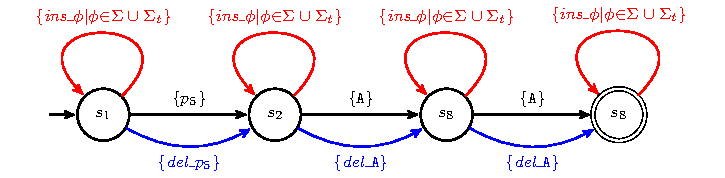
\includegraphics[width=.65\textwidth]{images/Tplus}}
	\caption{Augmented trace automaton $\mathcal{T}^+$ for $t_{\sigma'}=p_5\;\texttt{C}\;\texttt{C}$.}\label{fig:tplus}
\end{figure} \begin{figure}[!t]
\centering
{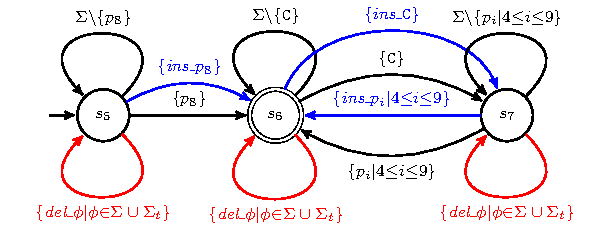
\includegraphics[width=.65\textwidth]{images/Aplus}}
\caption{Augmented constraint automaton $\mathcal{A}_{\varphi_{\mathcal{M}}}^+$ for $\mathcal{A}_{\varphi_{\mathcal{M}}}$.}\label{fig:aplus}
\end{figure}
Next, we augment $\mathcal{T}$ and $\mathcal{A}_{\varphi_{\mathcal{M}}}$ by adding transitions related to the atomic operations of insertions and deletions. Thus, from $\mathcal{T}$ we generate the automaton $\mathcal{T}^+=(\Sigma_t^+,Q_t,q_0^t,\rho_t^+,F_t)$ having:
\begin{itemize}
	\item $\Sigma_t^+$ extending $\Sigma_t\subseteq \Sigma$ by adding an insertion $\textit{ins\_}\phi$ for each atom $\phi\in\Sigma_t\cup\Sigma$ and a deletion $\textit{del\_}\phi$ for each atom  $\phi\in\Sigma_t$.
	\item $\rho_t^+$ extending $\rho_t$ by adding deletions $\rho_t^+(p,\textit{del\_}\phi)=q$ for each transition $\rho_t(p,\phi)=q$, and insertions $\rho_t^+(q,\textit{ins\_}\phi)=q$ for all atoms $\phi\in\Sigma\cup\Sigma_t$ and states $q\in Q_t$.
\end{itemize}
Figure~\ref{fig:tplus} shows the trace automaton generated from the deviant trace $\sigma_1$ from Example \ref{ex:first}. Similarly, from $\mathcal{A}_{\varphi_{\mathcal{M}}}$, we obtain $\mathcal{A}_{\varphi_{\mathcal{M}}}^+=(\Sigma^+,Q,q_0,\rho^+,F)$ having:
\begin{itemize}
	\item $\Sigma^+$ extending $\Sigma$ by adding an insertion $\textit{ins\_}\phi$ for each atom $\phi\in\Sigma$ and a deletion $\textit{del\_}\phi$ for each atom  $\phi\in\Sigma\cup\Sigma_t$.
\item $\rho^+$ extending $\rho_t$ by adding insertions $\rho^+(p,\textit{ins\_}\phi)=q$ for each transition $\rho(p,\phi)=q$ and deletions $\rho_t^+(q,\textit{del\_}\phi)=q$ for all atoms $\phi\in\Sigma\cup\Sigma_t$ and states $q\in Q$.
\end{itemize}
Figure~\ref{fig:aplus} shows the automaton augmented with the repair operations $\mathcal{A}_{\varphi_{\mathcal{M}}}^+$ obtained for the model $\mathcal{M}$ from Example \ref{ex:first}. Intuitively, $\mathcal{A}_{\varphi_{\mathcal{M}}}^+$ accepts all the string sequences conformant to the model and have been obtained by adding/removing the missing/wrong atoms to/from $t_\sigma$, where atomic operations are explicitly marked. As required, both augmented automata do not accept $t_{\sigma'}=p_5\;\texttt{C}\;\texttt{C}$. \added{If insertions are associated to the lowest cost, the best alignment strategy adds $p_8$ at the end on the trace; by  explicitly marking such repair  with $\textit{ins\_}p_8$, the augmented automata now accept $\hat{t_{\sigma'}}=p_5\;\texttt{C}\;\texttt{C}\;\textit{ins\_}p_8$. On the other hand, if re\-place\-ments are associated to the lowest cost, the best alignment strategy would replace the last \texttt{C} with $p_8$, thus requiring to first delete \texttt{C} and then insert $p_8$; the resulting $\hat{t_{\sigma'}}=p_5\;\texttt{C}\;\textit{del\_}p_8\;\textit{ins\_}p_8$ is also accepted by both automata}.

Next, we show how automated planners can efficiently identify the repair operations $\varrho$ needed to repair the trace $\sigma$ using the augmented automata just defined.

\subsection{Encoding in PDDL}\label{ssec:eip}

\newcommand{\myi}{\emph{(i)}\xspace}
\newcommand{\myii}{\emph{(ii)}\xspace}
\newcommand{\myiii}{\emph{(iii)}\xspace}
\newcommand{\myiv}{\emph{(iv)}\xspace}
\newcommand{\myv}{\emph{(v)}\xspace}
\newcommand{\myvi}{\emph{(vi)}\xspace}
\newcommand{\A}{\mathcal{A}}
\newcommand{\T}{\mathcal{T}}
\newcommand{\PDDL}[1]{\begin{footnotesize}\texttt{#1}\end{footnotesize}}
%E.g., the alignment result $\hat{t_\sigma}=p_5\;\texttt{A}\;\texttt{A}\;\textit{ins\_}p_8$ of trace $\sigma=$\texttt{B\{x=1,y=0\}A\{x=6\}\\A\{x=4\}} generates the repair $\varrho=[@\sigma_4\leftarrow p_8]$ after removing the \texttt{sync} operations.

\sloppypar

In this section, we show how, given an augmented constraint automaton $\mathcal{A}_{\varphi_{\mathcal{M}}}^+$ obtained from an LTL$_f$ formula  $\varphi_{\mathcal{M}}$, and an augmented trace automaton $\T^+$ obtained from a trace $t$, we build a cost-optimal planning domain $\mathcal{P_D}$ and a problem instance $\mathcal{P}$ in PDDL. $\mathcal{P_D}$ and $\mathcal{P}$ can be used to feed any state-of-the-art planners accepting PDDL 2.1 specifications, as discussed in Section \ref{ssec:ap}.
%
A solution plan for $\mathcal{P}$ amounts to the set of interventions of minimal cost to repair the trace with respect to $\varphi_{\mathcal{M}}'$.

%\paragraph{Planning Domain}
\medskip
\noindent
\textbf{Planning Domain.}
%
In $\mathcal{P_D}$, we provide two abstract types: \PDDL{activity} and \PDDL{state}.
%
The first captures the activities involved in a transition between two different states of a constraint/trace automaton.
%
The second is used to uniquely identify the states of the constraint automaton (through the sub-type \texttt{automaton\_state}) and of the trace automaton (through the sub-type \texttt{trace\_state}).
%
To capture the structure of the automaton and to monitor its evolution, we defined five \emph{domain propositions} as boolean predicates in $\mathcal{P_D}$:
%
\begin{itemize}
	\item \PDDL{(trace ?t1 - trace\_state ?e - activity ?t2 - trace\_state)} holds if there exists a transition in the trace automaton between two states \texttt{t1} and \texttt{t2}, being \texttt{e} the activity involved in the transition.
	\item \PDDL{(automaton ?s1 - automaton\_state ?e - activity ?s2 - automaton\_state)} holds if there exists a transition between two states \texttt{s1} to \texttt{s2} of a constraint automaton, being \texttt{e} the activity involved in the transition.
    \item \PDDL{(atoms ?e1 - activity ?e2 - activity)} holds if \texttt{e1} and \texttt{e2} are two atoms in $\Sigma$ associated to a same activity label.
	\item \PDDL{(cur\_state ?s - state)} holds if \texttt{s} is the current state of a constraint/trace automaton.
	\item \PDDL{(final\_state ?s - state)} holds if \texttt{s} is a final state of a constraint/trace automaton.
\end{itemize}
It is worth to notice that, if a generic activity \texttt{A} is associated to some data condition, \texttt{A} will be represented as a set of atoms $p_1$, $p_2$, $p_3$, etc. in $\mathcal{P_D}$, see for example Table \ref{tab:dimGMM}. This means that, for any combination of atoms $p_i$ - $p_j$ associated to \texttt{A}, there will exist an instance of the predicate \PDDL{(atoms)} that will hold for $p_i$ and $p_j$.
%
%Label \texttt{C} is never associated to a data condition, and therefore it will be associated to one single atom \texttt{C}. On the other hand, label \texttt{B} is associated to several atoms obtained by partitioning the data space via the intervals
%
Furthermore, we define a \emph{numeric fluent} \PDDL{total-cost} to keep track of the cost of the violations. Notice that: \myi in PDDL, parameters are written with a question mark character `?' in front, and the dash character `-' is used to assign types to parameters; and \myii we remain consistent with the PDDL syntax, which allows the values of both predicates and fluents to change as a result of the execution of an action.
%

Planning actions are used to express the \emph{repairs} on the original trace $t$. Each action is characterized by its \emph{preconditions} and \emph{effects}, stated in terms of the domain propositions. In our encoding, we have defined four actions to perform \emph{synchronous moves} both in the trace/constraint automaton, or to add/remove/replace activities to/from/in the constraint and trace automata. In the following, we suppose that actions \PDDL{ins}, \PDDL{del} and \PDDL{repl} have cost equal to 1. However, their cost can be customized to define the severity of a violation or to force priorities among actions.
%
%\begin{tiny}
%	\begin{verbatim}	
%	(:action sync                                          (:action add                              (:action del
%	:parameters (?t1 - path_state                           :parameters (?e - activity)               :parameters (?t1 - path_state
 %                ?e - activity                              :effect (and (increase (total-cost) 1)                  ?e - activity
  %               ?t2 - path_state)                           (forall (?s1 ?s2 - automaton_state)                    ?t2 - path_state)
%	:precondition (and (cur_state ?t1) (path ?t1 ?e ?t2))       (when (and (cur_state ?s1)            :precondition (and (cur_state ?t1)
%	:effect(and (not (cur_state ?t1)) (cur_state ?t2)           (automaton ?s1 ?e ?s2))               :effect(and (increase (total-cost) 1)
%	 (forall (?s1 ?s2 - automaton_state)                        (path ?t1 ?e ?t2))                    (not (cur_state ?t1)) (cur_state ?t2)))
%	   (when (and (cur_state ?s1)                               (and (not (cur_state ?s1))
%	   (automaton ?s1 ?e ?s2))                                  (cur_state ?s2))))))
%	   (and (not (cur_state ?s1))
%	   (cur_state ?s2))))))
%	\end{verbatim}
%\end{tiny}

\begin{scriptsize}
\begin{verbatim}
(:action sync
 :parameters (?t1 - trace_state ?e - activity ?t2 - trace_state)
 :precondition (and (cur_state ?t1) (trace ?t1 ?e ?t2))
 :effect(and (not (cur_state ?t1)) (cur_state ?t2)
             (forall (?s1 ?s2 - automaton_state)
               (when (and (cur_state ?s1)
                          (automaton ?s1 ?e ?s2))
                     (and (not (cur_state ?s1))(cur_state ?s2))))))

(:action ins                                     (:action del
 :parameters (?e - activity)                      :parameters (?t1 - trace_state
 :effect (and (increase (total-cost) 1)                        ?e - activity
          (forall (?s1 ?s2 - automaton_state)                  ?t2 - trace_state)
            (when (and (cur_state ?s1)            :precondition (and (cur_state ?t1)
                       (automaton ?s1 ?e ?s2))                     (trace ?t1 ?e ?t2))
                   (and (not (cur_state ?s1))     :effect(and (increase (total-cost) 1)
                        (cur_state ?s2))))))         (not (cur_state ?t1))(cur_state ?t2)))

(:action repl
 :parameters (?t1 - trace_state ?e1 - activity ?t2 - trace_state ?e2 - activity)
 :precondition (and (cur_state ?t1) (trace ?t1 ?e1 ?t2) (atoms ?e1 ?e2))
 :effect(and (increase (total-cost) 1) (not (cur_state ?t1)) (cur_state ?t2)
             (forall (?s1 ?s2 - automaton_state)
               (when (and (cur_state ?s1)
                          (automaton ?s1 ?e2 ?s2))
                     (and (not (cur_state ?s1))(cur_state ?s2))))))
\end{verbatim}
\end{scriptsize}
\smallskip

\noindent
We modeled \PDDL{sync} and \PDDL{del} in such a way that they can be applied only if there exists a transition from the current state \PDDL{t1} of the trace automaton to a subsequent state \PDDL{t2}, being \PDDL{e} the activity involved in the transition.
%%
Notice that, while \PDDL{del} yields a \emph{single} move in the trace automaton, \PDDL{sync} yields, in addition, one move on the constraint automaton, to be performed synchronously. In particular, a synchronous move is performed in the constraint automaton if there exists a transition involving activity \PDDL{e} connecting \PDDL{s1} -- the current state of the automaton -- to a state \PDDL{s2}.
%
Then, \PDDL{ins} is performed only for transitions involving activity \PDDL{e} connecting two states of the constraint automaton, with the current state of the trace automaton that remains the same after the execution of the action.
%
Finally, \PDDL{repl} can be seen as a synchronous combination of a \PDDL{del} and an \PDDL{ins}. It yields one move on the trace automaton and one on the constraint automaton, involving two atoms \PDDL{e1} and \PDDL{e2} associated to a same activity label, i.e., such that the predicate \PDDL{(atoms ?e1 ?e2)} holds.

\smallskip
\noindent
\textbf{Planning Problem.}
%\paragraph{Planning Problem}
%
In $\mathcal{P}$, we first define a finite set of constants required to properly ground all the domain propositions defined in $\mathcal{P_D}$. In our case, constants correspond to the state and activity instances involved in the trace/constraint automaton.
%
Secondly, we define the \emph{initial state} of $\mathcal{P}$ to capture the exact structure of the trace/constraint automaton. This includes the specification of all the existing transitions that connect two states of the automaton, and the definition of all the pairs of atoms belonging to a same activity label. The current state and the final states of the trace/constraint automaton are identified as well.
%
Thirdly, to encode the goal condition, we first pre-process the constraint automaton by: \myi adding a new dummy state with no outgoing transitions; \myii adding a new special action, executable only in the final states of the original automaton, which makes the automaton move to the dummy state; and \myiii including in the set of final states only the dummy state. Then, we define the goal condition as the conjunction of the final states of the trace automaton and of the constraint automaton. In this way, we avoid using disjunctions in goal formulas, which are not supported by all planners.
%
Finally, as our purpose is to minimize the total cost of the plan, $\mathcal{P}$ contains the following specification: \PDDL{(:metric minimize (total-cost))}. 


\subsection{Trace Repair}\label{ssec:trerepair}


Last, we need to leverage the repair actions generated by the planner to repair the \added{entire} trace \added{so to make it conformant to the model as a whole}. In particular, the generated repair actions are always ordered based on their positions within the trace. By removing all the \texttt{sync} actions provided by the planner, we will obtain a sequence of insertions $[@\texttt{t1}\leftarrow \texttt{e}]$, deletions $[\#\texttt{t1}\leftarrow \texttt{e}]$, and replacements $[\texttt{t1}[ \texttt{e1}\mapsto  \texttt{e2}]]$ for a trace $\sigma$ via its associated $t_\sigma$. While deletions $[\#\texttt{t1}\leftarrow \texttt{e}]$ can be trivially implemented in the data-aware scenario by simply removing the problematical event, %\deleted{at position $k$ from $\sigma$},
for insertions (or replacements), we need to add events with their associated payloads (or adapt the contained data values). Replacements $[\texttt{t1}[\texttt{e1}\mapsto  \texttt{e2}]]$ can be implemented by replacing the values in $\texttt{t1}$ violating the data condition $\texttt{e2}$ with the nearest values to the values in $\texttt{t1}$ satisfying $\texttt{e2}$. On the other hand, insertions require to generate totally new values: the insertion $[@\texttt{t1}\leftarrow \texttt{e}]$ of a new event $\texttt{t1}$ satisfying $\texttt{e}$ can be modeled by generating a new event having the label induced by $\texttt{e}$, which is then instantiated with the same data values present in the last occurrence of an event similarly labeled if any, and instantiated with default values otherwise; then, such values are repaired by choosing the values satisfying $\texttt{e}$ nearest to the default ones.
%
E.g., the alignment result $\hat{t_\sigma}=p_5\;\texttt{C}\;\texttt{C}\;\textit{ins\_}p_8$ of trace $\sigma=$\texttt{B\{x=1,y=0\}C\{x=6\}C\{x=4\}} generates the repair $\varrho=[@\sigma_4\leftarrow p_8]$ after removing the \texttt{sync} operations. Then, we obtain a new trace $\sigma=$\texttt{B\{x=1,y=0\}$  $C\{x=6\}C\{x=4\}B\{x=4,y=0\}}, where \texttt{4} is the nearest integer to \texttt{B.x=1} (taken from the first event) that satisfies $p_8\equiv\texttt{B}.x>3\wedge \texttt{B}.y=0$. 